%        File: doc.tex
%     Created: Sat Oct 26 03:00 AM 2013 E
% Last Change: Sat Oct 26 03:00 AM 2013 E
%
\documentclass[a4paper,12pt]{report}

% dot2tex
\usepackage[x11names, rgb]{xcolor}
%\usepackage{tikz}
%\usetikzlibrary{snakes,arrows,shapes}
\usepackage[utf8]{inputenc}
\usepackage{graphicx}
\usepackage[pdf]{pstricks}
\usepackage{amsmath}

\usepackage{pdfpages}

\usepackage[left=2.9cm,right=2.9cm,top=2cm,bottom=2cm]{geometry}
\usepackage[english,finnish]{babel}
\usepackage[T1]{fontenc}
\usepackage{lmodern}
\usepackage{setspace}\onehalfspacing
\usepackage{tabu}
\DeclareGraphicsRule{*}{mps}{*}{} % meta-uml

\newcommand{\HRule}{\rule{\linewidth}{0.5mm}}
\title{%
   \vspace{3cm}
   \textsc{\large Aineopintojen harjoitustyö: Tietokantasovellus \\ 2013/2\\}
   \HRule\\
   \textbf{\huge Kalenterijärjestelmä \\}
   \texttt{\large mustached-octo-happiness \\}
   \HRule
}
\author{%
   \begin{minipage}{0.95\textwidth}
      \begin{flushright}
         \large \emph{Tekijä}\\
         \large \textsc{Samuli Thomasson}
      \end{flushright}
   \end{minipage}
}
\date{\vfill \today}
\begin{document}

% Extra!! CryptoJS?

\maketitle
\tableofcontents
\chapter{Johdanto}
Tämä kalenterijärjestelmä mahdollistaa käyttäjille kalenterien yllä\-pidon
selaimesta.  Sovelluksen käyttäjä pystyy katsomaan, lisäämään
ja muokkaamaan (kalenteri)merkintöjä omissa kalentereissaan.  Kalenteri koostuu
joukosta merkintöjä, kuten tapahtumia ja muistutuksia.  Järjestelmä mahdollistaa
merkintöjen asettamisen julkisesti nähtäville. Myös kokonaisista kalentereista
voi tehdä julkisia. Julkisesta kalenterista voi myös tehdä vapaasti muokattavan,
jolloin kuka tahansa voi ehdottaa merkintöjä kalenteriin. Vapaasti muokattavassa
kalenterissa lopullinen määräysvalta on kalenterin omistajalla -- omistajan omia
tai hyväksymiä merkintöjä voi poistaa vain omistaja.

Järjestelmän toteutetuskieli on Haskell ja kehyksenä toimii \emph{Yesod}.
Järjestelmä on yksinkertaisuudessaan ohjelma, joka kuuntelee jossain portissa
web-palvelimena. Sitä voi siis ajaa itsenäisenä web-palvelimena suoraan portissa
80. Yleensä samankaltaiset sovellukset kuitenkin ajetaan paikallisessa portissa
ja välitetään dedikoidun web-palvelimen (Nginx ja vastaavat) kautta.

Järjestelmän alustajärjestelmältä vaaditaan, että lähdekoodi voidaan kääntää
sille. Staattisten kirjastojen ansoista ei käyttöönotto vaadi alustalta kuin
käännetyn ohjelman ajamisen, staattiset verkkosivuresurssit (JavaScript ja CSS)
sekä tuetun tietokannan. Ohjelma pitää ajaa omassa portissaan, eli ohjelman
käyttö vaatii joko ainoan web-palvelimen aseman ulkoisessa portissa, tai
(parempi) käänteisproxyä ymmärtävän web-palvelimen alustalta.

Järjestelmä suunnitellaan PostgreSQL-kannalle; vaihdon edellytyksiä on että
persistent tukee sitä, ja että tekijä ei ole käyttänyt liian erikoisia
SQL-konstruktioita.  Itse järjestelmän ominaisuuksien käyttöön asiakasohjelmassa
ei tarvitse JavaScriptiä. JavaScriptiä voidaan kuitenkiin käyttää
käyttökokemuksen parantamiseksi.

%%%%%%%%%%%%%%%%%%%%%%%%%%%%%%%%%%%%%%%%%%%%%%%%%%%%%%%%%%
\chapter{Järjestelmä}
\section{Yleiskuva järjestelmästä}
Käyttäjät toimivat aina selainkäyttöliittymän kautta. Käyttätapauskaaviossa
(\ref{graph_usecases}) on esitelty ohjelman päätoiminnot. Ne on jaettu kolmeen
pääryhmään: käyttäjien autentikointi, operaatiot omassa kalenterissa ja
operaatiot jonkun muun kalenterissa.

Järjestelmän käyttäjiä on kahdenlaisia: vierailijoita ja varsinaisia
käyttäjiä:
\begin{description}
   \item[Vierailijoita] ovat kaikki jotka eivät ole kirjautuneet sisään,
      riippumatta siitä onko heillä tunnisteita järjestelmässä vai ei.
   \item[Käyttäjiä] ovat kaikki sisäänkirjautuneet.
\end{description}

\section{Käyttötapaukset}
Tässä luvussa esitellään sovelluksen eri käyttötapaukset.  Ellei toisin mainita,
niin esiteltävät käyttö\-tapaukset ovat vain varsinaisille käyttäjille.
Käyttö\-tapaukset on jaettu kolmeen joukkoon: autentikointi, kalenterit
kohteineen ja vieraskalenterit.  Käyttö\-tapaus\-kaavio (\ref{graph_usecases})
havainnollistaa käyttötapauksiatapauksia; eri kategoriat on siinä jaettu
visaalisiin lohkoihin.
\begin{figure}[ht]
   \centering \includegraphics[width=\textwidth]{usecases.1}
   \caption{Kalenterijärjestelmän käyttötapauskaavio.
      \textcolor[rgb]{0.5,0.5,0}{Keltaisessa} laatikossa on autentikointi,
      \textcolor[rgb]{0,0.5,0.5}{turkoosissa} kalenterien ja kohteiden
      käyttötapaukset, ja
      \textcolor[rgb]{0.5,0,0.5}{violetissa} laatikossa on julkisten kalenterien
      käyttötapaukset.
   }
   \label{graph_usecases}
\end{figure}

\subsection{Autentikointi}
\begin{description}
   \item[Rekisteröityminen]  \emph{Vain vieraille}. Ensimmäinen asia jonka uuden
      tulevan käyt\-täjän täytyy valitettavasti tehdä, on rekisteröidä jokin
      tunniste itsestään järjes-telmään.  Tunniste on esimerkiksi
      sähköpostiosoite, jolla käyttäjä voi todentaa itsensä.

      Rekisteröitymiseen tarjotaan monia vaihtoehtoja. Perinteinen käyttäjänimen
      (sähköpostiosoitteen) ja salasanan tallennus palvelimelle on
      vakiovaihtoehto, mutta myös modernempia metodeja tarjotaan: BrowserId,
      OpenId ja Gmail, mahdollisesti muitakin.

   \item[Sisäänkirjautuminen]  \emph{Vain vieraille}. Käyttäjien täytyy pystyä
      autentikoimaan itsensä aiemmin ekiste\-röityneeksi käyttäjäksi
      (mahdollisesti itsekseen), eli järjes\-telmän kontekstissa korottamaan
      itsensä vieraasta käyttäjäksi.  Sisään\-kirjautumiseen käy\-tetään samaa
      metodia jota käyttäjä käytti rekisteröityessään.
\end{description}

\subsection{Kalenterit}\label{oma_kalenteri}
Käyttäjällä voi olla usea kalenteri järjestelmässä.  Käyttäjän luomaa kalenteria
kutsutaan \emph{käyttäjän omistamaksi} kalenteriksi.  Olemassaolevan kalenterin
omistajaa ei voi vaihtaa.  Omaan kalenteriin liittyvät toiminnot:
\begin{description}
   \item[Luonti] \hfill\\
      Kalenterin luominen on ensimmäinen asia jonka uusi
      käyttäjä tekee, ja se on helppoa: häneltä kysytään heti ensimmäisen
      sisäänkirjautumisen jälkeen nimeä kalenterille tekstikentällä.
      Kalenterille voi halutessaan asettaa jonkin toisen väriattribuutin kuin
      oletuksen.  Lisää attribuutteja voi varsinaisesti säätää myöhemmin, kun
      kalenteri on luotu (ks.\ kohta Muokkaus).

   \item[Tarkastelu {\it (kalenterinäkymä)}] \hfill\\
      Kalenterien tarkastelu on koko järjestelmän tärkein ja laajin
      käyttötapaus.  Sen voisi esittää myös useana pienempänä käyttötapauksena.

      Kalentereita ei pääasiassa tarkastella yksitellen, vaan useita
      päällekkäin.  Tarkastelu tapahtuu \emph{kalenterinäkymässä}.
      Kalenterinäkymässä näytetään kerrallaan yhden viikon tapahtumat
      kalentereista.\footnote{%
         Jos aikaa riittää niin näytettävä sisältö on paremmin säädettävissä
         (kuukausi, päivä, tai muita näkymiä).
      }  Näkyvää viikkoa voi vaihtaa seuraavaan, edelliseen, senhetkiseen
      viikkoon tai johonkin tiettyyn viikkoon.

      Näkymässä näkyvät kalenterit voi valita.

      Näkymässä on esillä keinoja kalenterikohteiden operointiin.  Näkyvistä
      kalenterikohteista näytetään lyhyet yhteenvedot sekä keinot niiden
      muokkaukseen.
   \item[Muokkaus {\it (kalenterin ominaisuudet)}] \hfill\\
      Kalenterit ovat vain kohteita kokoavia entiteettejä, mutta niillä on silti
      muutama muokattava attribuutti jotka vaikuttavat niiden toimintaan. Näitä
      ovat:
      \begin{description}
         \item[Nimi]  Kalenterin muista identifioiva tunniste.
         \item[Väri]  Minkä värisinä kalenterin kohteet näkyvät
            kalenterinäkymässä.
         \item[Julkinen]  Voiko kalenterin kohteita tarkastella kuka vain
            (käyttäjä tai vieras).
         \item[Yhteinen]  Voiko kuka vain lisätä kalenteriin omia kohteita.
            Selvästi tämä attribuutti on järkevä vain kun kalenteri on
            julkinen.  
      \end{description}

      Kaikkia attribuutteja voi muokata muokkaus\-näkymässä, jossa näkyvät myös
      nykyiset arvot.
   \item[Poisto] \hfill\\
      Kalenterin voi myös poistaa, ja sekin tapahtuu muokkausnäkymässä.
      Poistoon kysytään varmistus mikäli kalenteri sisältää kohteita, sillä
      kohteet poistuvat myös.
\end{description}

\subsection{Kalenterikohteet}
Kalenterit koostuvat erilaisista (kalenteri)kohteista.  Kaikille erilaisista
kohteista on samantapaiset käyttöliittymät, joissa keskinäiset erot muodostuvat
kohdetyyppien erilaisista tietokentistä.  Yhteisiä ominaisuuksia, kuten
päivämääriä operoidaan samoin kohdetyypistä riippumatta.  Lisäksi jokaisesta
kohteesta tallennetaan metadataa, kuten luonti- ja muokkauspäivämääriä.

Yleiseen kalenterikohteeseen liittyvät käyttötapaukset:
\begin{description}
   \item[Luonti]\hfill\\
      Kalenterikohteita lisätään valitsemalla haluttu kohdetyyppi
      kalenteri\-näky\-mäs\-sä. Kalenterinäkymässä voi kohteen lisäykseen edetä joko
      tietylle ajalle aikanäkymässä (viikkonäkymässä), tai aikanäkymän
      ulkopuolelta.

   \item[Tarkastelu]\hfill\\
      Kalenterikohteita tarkastellaan kalenterinäkymässä, ja kohteiden
      yksityiskohtia valitsemalla kohteen kalenterinäkymässä.

   \item[Muokkaus]\hfill\\
      Kohteen muokkaukseen edetään sen yksityiskohtaisesta näkymästä.
      Muokattavia attribuutteja on useita ja ne riippuvat kohdetyypistä.
      Kaikista kohteista muokattavat attribuutit:
      \begin{description}
         \item[Kuvaus]  Tärkein attribuutti on kuvaus kohteesta.
         \item[Paikka]  Kohteeseen liittyvä maantieteellinen sijainti.
         \item[Kommentti]  Sivuhuomautus kohteesta.
         \item[Osallistujat] Henkilöt, joita kohde koskee.
         \item[Tärkeys]  Kuinka tärkeä kohde on (jollain asteikolla).
         \item[Hälytysajat]  Kun kohteesta halutaan muistutus. Esimerkiksi
            tietty aika ennen tapahtuman alkamisajankohtaa tai to-do:n
            deadlinea.
      \end{description}

      Kohteiden metadata (luodaan implisiittisesti):
      \begin{description}
         \item[Luontipäivämäärä]  Jotta voidaan tarkistaa koska kohde lisättiin
            kalenteriin.
         \item[Viimeinen muokkaus]  Koska edellinen muokkaus tehtiin?
      \end{description}

      Kohdetyypeille ominaiset muokattavat attribuutit:
      \\(Nämä muistuttavat (hyvin löyhästi) iCalendar-määrittelyä)
      \begin{description}
         \item[Tapahtuma (VEVENT)] \hfill\\
            Kalenterien tyypillinen ominaisuus on tapahtumien muistaminen ja
            niistä muistuttaminen. Tärkeimmät attribuutit:
            \begin{description}
               \item[Alkamisajankohta]  Koska tapahtuma alkaa?
               \item[Kesto]  Kauanko tapahtuma kestää?
               \item[Toistuvuus] Kuinka usein ja milloin tapahtuma toistuu (jos
                  toistuu)?
            \end{description}

         \item[Muistiinpano (VJOURNAL)] \hfill\\
            Muistiinpanot ovat yleiskäyttöisiä
            kohteita.  Niitä voi käyttää esimerkiksi päiväkirjana tai
            mikroblogina. Attribuutit:
            \begin{description}
               \item[Sisältö] Yleisen kohteen kuvauksesta eroava, rikkaampi
                  kenttä. Sisältö voi olla esimerkiksi HTML:ää tai Markdown:ia.
            \end{description}

         \item[To-do (VTODO)] \hfill\\
            To-do:n voi tehdä mistä tahansa tehtävästä. Attribuutit:
            \begin{description}
               \item[Valmis] Onko \texttt{todo} valmistunut?
               \item[Toistuvuus] Toistuuko tehtävä säännöllisesti, milloin?
            \end{description}
      \end{description}

   \item[Kopiointi]\hfill\\
      Kohteista voi luoda kopioita, tai tarkemmin olemassa\-olevaa kohdetta voi
      läh\-teä muokkaamaan ja tallentaa muokattu versio uutena kohteena. Tämäkin
      tapahtuu yksityiskohtaisesta näkymästä.

   \item[Poisto]\hfill\\
      Kohteen poisto tapahtuu myös sen yksityiskohtaisesta näkymästä.  Poistoon
      kysytään aina varmistus.  Toistuvien kohteiden kohdalla kysytään,
      halutaanko poistaa kaikki toistot vai ainoastaan valittu toisto.

   \item[Jako]\hfill\\
      Yksittäisiä kohteita voi jakaa sellaisenaan muille järjestelmän
      käyttäjille, ja myös viedä tekstimuotoon esimerkiksi liitettäväksi
      sähköpostiin.  Jakamiseen edetään yksityiskohtaisesta näkymästä. 

      Toiselle käyttäjälle kohdistuvalle jaolle annetaan käyttäjäjoukko, jotka
      saavat heille jaetusta kohteesta ilmoituksen.  He päättävät haluavatko
      lisätä kohteen johonkin omaan kalenteriin.
\end{description}

\subsection{Vieraskalenterit}
Vieraskalenteri-käyttötapaukset koskevat käyttäjiä, vieraita ja niitä
kalentereita jotka eivät ole heidän omistamia.  Vieraskalenteria pystyy
tarkastelemaan ja mahdollisesti (omistajan niin asettaessa) tekemään lisäyksiä,
mutta \emph{ei} muutoksia kalenteriin tai siinä oleviin muiden omistamiin
kalenterikohteisiin.  Näiden käyttötapausten oletus on, että kohteena olevan
kalenterin omistaja on sallinut julkiset toiminnot.  Käyttötapaukset:
\begin{description}
   \item[Tarkastelu]\hfill\\
      \textit{Kaikille} Vieraskalenteria voi tarkastella samalla tavalla kuin
      omaakin kalenteria (ks.~\ref{oma_kalenteri}).
   \item[Kohteen luonti]\hfill\\
      \textit{Kaikille}. Vieraskalenteriin voi lisätä kohteita jos kalenterin
      omistaja on sen sallinut.  Lisäys tapahtuu samalla tavalla kuin oman
      kalenterin tapauksessa. 

      Vieraalta saatetaan vaatia kuva- tai muu varmennus (captcha).
\end{description}

\section{Järjestelmän tietosisältö}
Järjestelmän tietokohteet on esitetty pääpiirteittäin
kaaviossa~\ref{graph_class}. Tietosisällöt on kuvattu yksityiskohtaisemmin
alaluvuissa. Taulukoissa on esitetty kunkin tietokohteet attribuuttien nimet,
arvojoukot ja kuvaukset. Attribuutti on pakollinen ellei arvojoukkoon ole
merkattu (V). Listattujen attribuuttien lisäksi myös metatiedot (koska luotu,
koska viimeksi muokattu) tallennetaan.

\begin{figure}[ht]
   \centering \includegraphics[width=\textwidth]{class.1}
   \caption{Käsitekaavio järjestelmän tietokohteista. Harmaaseen laatikkoon
   osoittavat relaatiot liittyvät jokaiseen kohteeseen laatikossa.}
   \label{graph_class}
\end{figure}

\newenvironment{tietokohde}
   {\medskip\noindent\begin{tabu}to\linewidth%
         {|X[-1,l]|X[-1,l]|X[-1,l]<{\strut}|}
         \hline
         \rowfont{\bfseries} Attribuutti & Arvojoukko & Kuvailu \\
         \hline
   }
   {\end{tabu}\medskip}

\subsection{Tietokohde: Kalenteri}

\begin{tietokohde}
   Omistaja              & Käyttäjä   & Kuka loi ja omistaa kalenterin. \\\hline
   Nimi                  & Merkkijono & Nimi ja samalla tunniste kalenterille. \\\hline
   Kuvaus                & Merkkijono (V) & Lisätietoa kalenterista. \\\hline
   Väri                  & Merkkijono (RGB) & Tunnisteväri kalenterin kohteille. \\\hline
   Onko julkinen         & Totuusarvo & Voiko kalenteria katsoa kuka vain? \\\hline
   Julkisesti muokattava & Totuusarvo & Voiko kohteita lisätä kuka vain? \\\hline
\end{tietokohde}

\noindent
Kalenteriin kuuluu useita kalenterikohteita. Kalenteri kuuluu yhdelle
käyttäjälle, omistajalle.

\subsection{Kalenterikohteet}\label{kohteet_kohde}

Kaikille kalenterikohteille tyypilliset attribuutit:

\begin{tietokohde}
   Omistaja    & Käyttäjä         & Kohteen luoja ja omistaja. \\\hline
   Nimi        & Merkkijono       & Nimike kohteelle. \\\hline
\end{tietokohde}

\noindent
Jokainen kalenterikohde on yhden käyttäjän omistuksessa, mutta voi olla useassa,
myös toisen käyttäjän kalenterissa. Kohteet kuuluvat aina vähintään yhteen
kalenteriin, eli \textbf{kalenterikohde ei voi olla orpo}.

\textit{Tärkeys} ilmaistaan neliportaisella asteikolla: joutava, normaali,
tärkeä tai kriittinen.
\textit{Henkilöt} voivat viitata niin järjestelmän käyttäjiin kuin ulkopuolisiin
kontakteihin (nimi, sähköposti jne.); käytännössä merkkijonoja.

\subsubsection{Tietokohde: Muistiinpano}

\begin{tietokohde}
   \multicolumn{3}{|c|}{(Taulukon~\ref{kohteet_kohde} attribuutit)} \\\hline
   Sisältö & \textit{Rikas teksti} & Muistiinpanon sisältö. \\\hline
\end{tietokohde}

\noindent
\textit{Rikas teksti} on joko paljasta tekstiä, tai
markdownia.\footnote{Riippuen aikataulusta}

\subsubsection{Tietokohde: To-do}
\begin{tietokohde}
   \multicolumn{3}{|c|}{(Taulukon~\ref{kohteet_kohde} attribuutit)} \\\hline

   Valmis     & Totuusarvo      & Onko to-do jo tehty? \\\hline
   Toistuvuus & \textit{Toisto} & Mihin aikaan, miten toistuu? \\\hline
   AlkuPvm    & Päivämäärä      & Mistä alkaen kohde on relevantti? \\\hline
   ViimPvm    & Päivämäärä (V)  & Mistä alkaen kohde on vanhentunut? \\\hline
   Hälytys    & Aikaero         & Halutaanko ennen deadlinea hälytys?  \\\hline
   Tärkeysaste & \textit{Tärkeys} & Kuinka kriittinen kohde on. \\\hline
\end{tietokohde}

\noindent
\textit{Toisto} kertoo ajankohdan jolloin tehtävän on oltava tehty (deadline),
ja mahdollisesti myös kuinka useasti (päivittäin, viikoittain, kuukausittain,
\ldots) kohde toistuu ja mihin asti toisto jatkuu.

\subsubsection{Tietokohde: Tapahtuma}
\begin{tietokohde}
   \multicolumn{3}{|c|}{(Taulukon~\ref{kohteet_kohde} attribuutit)} \\\hline

   Toistuvuus  & Toisto      & Mihin aikaan, miten toistuu? \\\hline
   AlkuPvm     & Päivämäärä  & Mistä alkaen kohde on relevantti? \\\hline
   ViimPvm     & Päivämäärä (V) & Mistä alkaen kohde on vanhentunut? \\\hline
   Paikka      & Merkkijono (V)   & Kohteeseen liittyvä sijainti. \\\hline
   Tärkeysaste & \textit{Tärkeys} & Kuinka kriittinen kohde on. \\\hline
   Hälytys     & Aikaero (V) & Halutaanko ennen tapahtumaa hälytys? \\\hline
   Osallistujat& \textit{Henkilöt} (V) & Kohteeseen liittyvät henkilöt. \\\hline
   Kuvaus      & Merkkijono (V)   & Huomautus kohteesta. \\\hline
\end{tietokohde}

\section{Relaatiotietokanta}
Järjestelmän tietokannan taulut ja niiden pää- ja vierasavaimet on kuvattu
kaaviossa~\ref{graph_database}. Taulukossa~\ref{graph_columns} on lueteltu
taulujen sarakkeet ja niiden tyypit kannassa. Todellisuudessa kanta on luotu ja
käytetään jarjestelmässä \texttt{persistent}-kirjaston avulla, ks. tiedosto
\texttt{config/models}.
\begin{figure}[hb]
   \centering
\begin{pspicture}[linewidth=1bp](0bp,0bp)(288bp,468bp)

  \pstVerb{2 setlinejoin} % set line join style to 'mitre'
%%
{
  \psset{linecolor=[rgb]{0.0,0.0,0.0}}
}
  \psset{linecolor=black}
  % Edge: todo -> target
  \psbezier[arrows=<-](224bp,82bp)(144.01bp,105.43bp)(257.32bp,288bp)(168bp,288bp)
  % Edge: calendar -> user
  \psbezier[arrows=<-](106bp,400bp)(58.072bp,375.85bp)(114.44bp,270bp)(59bp,270bp)
  % Edge: cal_target -> calendar
  \psbezier[arrows=<-](218bp,418bp)(192.55bp,418bp)(185.5bp,418bp)(170bp,418bp)
  % Edge: note -> target
  \psbezier[arrows=<-](224bp,194bp)(184.04bp,215.39bp)(210.74bp,288bp)(168bp,288bp)
  % Edge: email -> user
  \psbezier[arrows=<-](113bp,140bp)(62.597bp,163.23bp)(115.7bp,270bp)(59bp,270bp)
  % Edge: target -> user
  \psbezier[arrows=<-](108bp,270bp)(82.177bp,270bp)(74.993bp,270bp)(59bp,270bp)
  % Edge: cal_target -> target
  \psbezier[arrows=<-](218bp,400bp)(175.04bp,376.84bp)(216.55bp,288bp)(168bp,288bp)
  % Edge: event -> target
  \psbezier[arrows=<-](224bp,306bp)(195.16bp,298.99bp)(188.42bp,288bp)(168bp,288bp)
  % Node: target
{%
  \psset{linecolor=[rgb]{1.0,1.0,1.0}}
  \psset{fillcolor=[rgb]{1.0,1.0,1.0}}
  \psset{fillcolor=[rgb]{0.61,0.67,0.59}}
  \pspolygon[fillstyle=solid](109bp,297bp)(109bp,316bp)(167bp,316bp)(167bp,297bp)
  \psset{linecolor=[rgb]{0.0,0.0,0.0}}
  \pspolygon[](109bp,297bp)(109bp,316bp)(167bp,316bp)(167bp,297bp)
  \rput[l](124bp,303.7bp){target}
  \psset{linecolor=[rgb]{1.0,1.0,1.0}}
  \psset{fillcolor=[rgb]{0.75,0.82,0.72}}
  \pspolygon[fillstyle=solid](109bp,279bp)(109bp,297bp)(167bp,297bp)(167bp,279bp)
  \psset{linecolor=[rgb]{0.0,0.0,0.0}}
  \pspolygon[](109bp,279bp)(109bp,297bp)(167bp,297bp)(167bp,279bp)
  \rput[l](112bp,285.2bp){id}
  \pspolygon[](109bp,261bp)(109bp,279bp)(167bp,279bp)(167bp,261bp)
  \rput[l](112bp,267.2bp){owner}
  \pspolygon[](109bp,243bp)(109bp,261bp)(167bp,261bp)(167bp,243bp)
  \rput[l](112bp,249.2bp){...}
  \psset{linecolor=[rgb]{1.0,1.0,1.0}}
  \psset{fillcolor=[rgb]{0.97,0.97,0.97}}
  \pspolygon[fillstyle=solid](109bp,225bp)(109bp,243bp)(132bp,243bp)(132bp,225bp)
  \psset{linecolor=[rgb]{0.0,0.0,0.0}}
  \pspolygon[](109bp,225bp)(109bp,243bp)(132bp,243bp)(132bp,225bp)
  \rput[l](112bp,231.2bp){< 1}
  \psset{linecolor=[rgb]{1.0,1.0,1.0}}
  \pspolygon[fillstyle=solid](132bp,225bp)(132bp,243bp)(145bp,243bp)(145bp,225bp)
  \psset{linecolor=[rgb]{0.0,0.0,0.0}}
  \pspolygon[](132bp,225bp)(132bp,243bp)(145bp,243bp)(145bp,225bp)
  \rput[l](135bp,231.2bp){  }
  \psset{linecolor=[rgb]{1.0,1.0,1.0}}
  \pspolygon[fillstyle=solid](145bp,225bp)(145bp,243bp)(167bp,243bp)(167bp,225bp)
  \psset{linecolor=[rgb]{0.0,0.0,0.0}}
  \pspolygon[](145bp,225bp)(145bp,243bp)(167bp,243bp)(167bp,225bp)
  \rput[l](148bp,231.2bp){4 >}
}%
  % Node: email
{%
  \psset{linecolor=[rgb]{1.0,1.0,1.0}}
  \psset{fillcolor=[rgb]{1.0,1.0,1.0}}
  \psset{fillcolor=[rgb]{0.61,0.67,0.59}}
  \pspolygon[fillstyle=solid](114bp,185bp)(114bp,204bp)(163bp,204bp)(163bp,185bp)
  \psset{linecolor=[rgb]{0.0,0.0,0.0}}
  \pspolygon[](114bp,185bp)(114bp,204bp)(163bp,204bp)(163bp,185bp)
  \rput[l](125bp,191.7bp){email}
  \psset{linecolor=[rgb]{1.0,1.0,1.0}}
  \psset{fillcolor=[rgb]{0.75,0.82,0.72}}
  \pspolygon[fillstyle=solid](114bp,167bp)(114bp,185bp)(163bp,185bp)(163bp,167bp)
  \psset{linecolor=[rgb]{0.0,0.0,0.0}}
  \pspolygon[](114bp,167bp)(114bp,185bp)(163bp,185bp)(163bp,167bp)
  \rput[l](117bp,173.2bp){id}
  \psset{linecolor=[rgb]{1.0,1.0,1.0}}
  \psset{fillcolor=[rgb]{0.96,0.97,0.85}}
  \pspolygon[fillstyle=solid](114bp,149bp)(114bp,167bp)(163bp,167bp)(163bp,149bp)
  \psset{linecolor=[rgb]{0.0,0.0,0.0}}
  \pspolygon[](114bp,149bp)(114bp,167bp)(163bp,167bp)(163bp,149bp)
  \rput[l](117bp,155.2bp){email}
  \pspolygon[](114bp,131bp)(114bp,149bp)(163bp,149bp)(163bp,131bp)
  \rput[l](117bp,137.2bp){user}
  \pspolygon[](114bp,113bp)(114bp,131bp)(163bp,131bp)(163bp,113bp)
  \rput[l](117bp,119.2bp){...}
  \psset{linecolor=[rgb]{1.0,1.0,1.0}}
  \psset{fillcolor=[rgb]{0.97,0.97,0.97}}
  \pspolygon[fillstyle=solid](114bp,95bp)(114bp,113bp)(137bp,113bp)(137bp,95bp)
  \psset{linecolor=[rgb]{0.0,0.0,0.0}}
  \pspolygon[](114bp,95bp)(114bp,113bp)(137bp,113bp)(137bp,95bp)
  \rput[l](117bp,101.2bp){< 1}
  \psset{linecolor=[rgb]{1.0,1.0,1.0}}
  \pspolygon[fillstyle=solid](137bp,95bp)(137bp,113bp)(150bp,113bp)(150bp,95bp)
  \psset{linecolor=[rgb]{0.0,0.0,0.0}}
  \pspolygon[](137bp,95bp)(137bp,113bp)(150bp,113bp)(150bp,95bp)
  \rput[l](140bp,101.2bp){  }
  \psset{linecolor=[rgb]{1.0,1.0,1.0}}
  \pspolygon[fillstyle=solid](150bp,95bp)(150bp,113bp)(163bp,113bp)(163bp,95bp)
  \psset{linecolor=[rgb]{0.0,0.0,0.0}}
  \pspolygon[](150bp,95bp)(150bp,113bp)(163bp,113bp)(163bp,95bp)
  \rput[l](153bp,101.2bp){}
}%
  % Node: note
{%
  \psset{linecolor=[rgb]{1.0,1.0,1.0}}
  \psset{fillcolor=[rgb]{1.0,1.0,1.0}}
  \psset{fillcolor=[rgb]{0.61,0.67,0.59}}
  \pspolygon[fillstyle=solid](225bp,221bp)(225bp,240bp)(274bp,240bp)(274bp,221bp)
  \psset{linecolor=[rgb]{0.0,0.0,0.0}}
  \pspolygon[](225bp,221bp)(225bp,240bp)(274bp,240bp)(274bp,221bp)
  \rput[l](238.5bp,227.7bp){note}
  \psset{linecolor=[rgb]{1.0,1.0,1.0}}
  \psset{fillcolor=[rgb]{0.75,0.82,0.72}}
  \pspolygon[fillstyle=solid](225bp,203bp)(225bp,221bp)(274bp,221bp)(274bp,203bp)
  \psset{linecolor=[rgb]{0.0,0.0,0.0}}
  \pspolygon[](225bp,203bp)(225bp,221bp)(274bp,221bp)(274bp,203bp)
  \rput[l](228bp,209.2bp){id}
  \pspolygon[](225bp,185bp)(225bp,203bp)(274bp,203bp)(274bp,185bp)
  \rput[l](228bp,191.2bp){target}
  \pspolygon[](225bp,167bp)(225bp,185bp)(274bp,185bp)(274bp,167bp)
  \rput[l](228bp,173.2bp){...}
  \psset{linecolor=[rgb]{1.0,1.0,1.0}}
  \psset{fillcolor=[rgb]{0.97,0.97,0.97}}
  \pspolygon[fillstyle=solid](225bp,149bp)(225bp,167bp)(248bp,167bp)(248bp,149bp)
  \psset{linecolor=[rgb]{0.0,0.0,0.0}}
  \pspolygon[](225bp,149bp)(225bp,167bp)(248bp,167bp)(248bp,149bp)
  \rput[l](228bp,155.2bp){< 1}
  \psset{linecolor=[rgb]{1.0,1.0,1.0}}
  \pspolygon[fillstyle=solid](248bp,149bp)(248bp,167bp)(261bp,167bp)(261bp,149bp)
  \psset{linecolor=[rgb]{0.0,0.0,0.0}}
  \pspolygon[](248bp,149bp)(248bp,167bp)(261bp,167bp)(261bp,149bp)
  \rput[l](251bp,155.2bp){  }
  \psset{linecolor=[rgb]{1.0,1.0,1.0}}
  \pspolygon[fillstyle=solid](261bp,149bp)(261bp,167bp)(274bp,167bp)(274bp,149bp)
  \psset{linecolor=[rgb]{0.0,0.0,0.0}}
  \pspolygon[](261bp,149bp)(261bp,167bp)(274bp,167bp)(274bp,149bp)
  \rput[l](264bp,155.2bp){}
}%
  % Node: user
{%
  \psset{linecolor=[rgb]{1.0,1.0,1.0}}
  \psset{fillcolor=[rgb]{1.0,1.0,1.0}}
  \psset{fillcolor=[rgb]{0.61,0.67,0.59}}
  \pspolygon[fillstyle=solid](9bp,279bp)(9bp,298bp)(58bp,298bp)(58bp,279bp)
  \psset{linecolor=[rgb]{0.0,0.0,0.0}}
  \pspolygon[](9bp,279bp)(9bp,298bp)(58bp,298bp)(58bp,279bp)
  \rput[l](22.5bp,285.7bp){user}
  \psset{linecolor=[rgb]{1.0,1.0,1.0}}
  \psset{fillcolor=[rgb]{0.75,0.82,0.72}}
  \pspolygon[fillstyle=solid](9bp,261bp)(9bp,279bp)(58bp,279bp)(58bp,261bp)
  \psset{linecolor=[rgb]{0.0,0.0,0.0}}
  \pspolygon[](9bp,261bp)(9bp,279bp)(58bp,279bp)(58bp,261bp)
  \rput[l](12bp,267.2bp){id}
  \psset{linecolor=[rgb]{1.0,1.0,1.0}}
  \psset{fillcolor=[rgb]{0.96,0.97,0.85}}
  \pspolygon[fillstyle=solid](9bp,243bp)(9bp,261bp)(58bp,261bp)(58bp,243bp)
  \psset{linecolor=[rgb]{0.0,0.0,0.0}}
  \pspolygon[](9bp,243bp)(9bp,261bp)(58bp,261bp)(58bp,243bp)
  \rput[l](12bp,249.2bp){ident}
  \pspolygon[](9bp,225bp)(9bp,243bp)(58bp,243bp)(58bp,225bp)
  \rput[l](12bp,231.2bp){...}
  \psset{linecolor=[rgb]{1.0,1.0,1.0}}
  \psset{fillcolor=[rgb]{0.97,0.97,0.97}}
  \pspolygon[fillstyle=solid](9bp,207bp)(9bp,225bp)(23bp,225bp)(23bp,207bp)
  \psset{linecolor=[rgb]{0.0,0.0,0.0}}
  \pspolygon[](9bp,207bp)(9bp,225bp)(23bp,225bp)(23bp,207bp)
  \rput[l](12bp,213.2bp){  }
  \psset{linecolor=[rgb]{1.0,1.0,1.0}}
  \pspolygon[fillstyle=solid](23bp,207bp)(23bp,225bp)(36bp,225bp)(36bp,207bp)
  \psset{linecolor=[rgb]{0.0,0.0,0.0}}
  \pspolygon[](23bp,207bp)(23bp,225bp)(36bp,225bp)(36bp,207bp)
  \rput[l](26bp,213.2bp){  }
  \psset{linecolor=[rgb]{1.0,1.0,1.0}}
  \pspolygon[fillstyle=solid](36bp,207bp)(36bp,225bp)(58bp,225bp)(58bp,207bp)
  \psset{linecolor=[rgb]{0.0,0.0,0.0}}
  \pspolygon[](36bp,207bp)(36bp,225bp)(58bp,225bp)(58bp,207bp)
  \rput[l](39bp,213.2bp){3 >}
}%
  % Node: calendar
{%
  \psset{linecolor=[rgb]{1.0,1.0,1.0}}
  \psset{fillcolor=[rgb]{1.0,1.0,1.0}}
  \psset{fillcolor=[rgb]{0.61,0.67,0.59}}
  \pspolygon[fillstyle=solid](107bp,427bp)(107bp,446bp)(169bp,446bp)(169bp,427bp)
  \psset{linecolor=[rgb]{0.0,0.0,0.0}}
  \pspolygon[](107bp,427bp)(107bp,446bp)(169bp,446bp)(169bp,427bp)
  \rput[l](116.5bp,433.7bp){calendar}
  \psset{linecolor=[rgb]{1.0,1.0,1.0}}
  \psset{fillcolor=[rgb]{0.75,0.82,0.72}}
  \pspolygon[fillstyle=solid](107bp,409bp)(107bp,427bp)(169bp,427bp)(169bp,409bp)
  \psset{linecolor=[rgb]{0.0,0.0,0.0}}
  \pspolygon[](107bp,409bp)(107bp,427bp)(169bp,427bp)(169bp,409bp)
  \rput[l](110bp,415.2bp){id}
  \psset{linecolor=[rgb]{1.0,1.0,1.0}}
  \psset{fillcolor=[rgb]{0.96,0.97,0.85}}
  \pspolygon[fillstyle=solid](107bp,391bp)(107bp,409bp)(169bp,409bp)(169bp,391bp)
  \psset{linecolor=[rgb]{0.0,0.0,0.0}}
  \pspolygon[](107bp,391bp)(107bp,409bp)(169bp,409bp)(169bp,391bp)
  \rput[l](110bp,397.2bp){owner}
  \psset{linecolor=[rgb]{1.0,1.0,1.0}}
  \pspolygon[fillstyle=solid](107bp,373bp)(107bp,391bp)(169bp,391bp)(169bp,373bp)
  \psset{linecolor=[rgb]{0.0,0.0,0.0}}
  \pspolygon[](107bp,373bp)(107bp,391bp)(169bp,391bp)(169bp,373bp)
  \rput[l](110bp,379.2bp){name}
  \pspolygon[](107bp,355bp)(107bp,373bp)(169bp,373bp)(169bp,355bp)
  \rput[l](110bp,361.2bp){...}
  \psset{linecolor=[rgb]{1.0,1.0,1.0}}
  \psset{fillcolor=[rgb]{0.97,0.97,0.97}}
  \pspolygon[fillstyle=solid](107bp,337bp)(107bp,355bp)(130bp,355bp)(130bp,337bp)
  \psset{linecolor=[rgb]{0.0,0.0,0.0}}
  \pspolygon[](107bp,337bp)(107bp,355bp)(130bp,355bp)(130bp,337bp)
  \rput[l](110bp,343.2bp){< 1}
  \psset{linecolor=[rgb]{1.0,1.0,1.0}}
  \pspolygon[fillstyle=solid](130bp,337bp)(130bp,355bp)(147bp,355bp)(147bp,337bp)
  \psset{linecolor=[rgb]{0.0,0.0,0.0}}
  \pspolygon[](130bp,337bp)(130bp,355bp)(147bp,355bp)(147bp,337bp)
  \rput[l](137bp,343.2bp){  }
  \psset{linecolor=[rgb]{1.0,1.0,1.0}}
  \pspolygon[fillstyle=solid](147bp,337bp)(147bp,355bp)(169bp,355bp)(169bp,337bp)
  \psset{linecolor=[rgb]{0.0,0.0,0.0}}
  \pspolygon[](147bp,337bp)(147bp,355bp)(169bp,355bp)(169bp,337bp)
  \rput[l](150bp,343.2bp){1 >}
}%
  % Node: todo
{%
  \psset{linecolor=[rgb]{1.0,1.0,1.0}}
  \psset{fillcolor=[rgb]{1.0,1.0,1.0}}
  \psset{fillcolor=[rgb]{0.61,0.67,0.59}}
  \pspolygon[fillstyle=solid](225bp,109bp)(225bp,128bp)(274bp,128bp)(274bp,109bp)
  \psset{linecolor=[rgb]{0.0,0.0,0.0}}
  \pspolygon[](225bp,109bp)(225bp,128bp)(274bp,128bp)(274bp,109bp)
  \rput[l](238.5bp,115.7bp){todo}
  \psset{linecolor=[rgb]{1.0,1.0,1.0}}
  \psset{fillcolor=[rgb]{0.75,0.82,0.72}}
  \pspolygon[fillstyle=solid](225bp,91bp)(225bp,109bp)(274bp,109bp)(274bp,91bp)
  \psset{linecolor=[rgb]{0.0,0.0,0.0}}
  \pspolygon[](225bp,91bp)(225bp,109bp)(274bp,109bp)(274bp,91bp)
  \rput[l](228bp,97.2bp){id}
  \pspolygon[](225bp,73bp)(225bp,91bp)(274bp,91bp)(274bp,73bp)
  \rput[l](228bp,79.2bp){target}
  \pspolygon[](225bp,55bp)(225bp,73bp)(274bp,73bp)(274bp,55bp)
  \rput[l](228bp,61.2bp){...}
  \psset{linecolor=[rgb]{1.0,1.0,1.0}}
  \psset{fillcolor=[rgb]{0.97,0.97,0.97}}
  \pspolygon[fillstyle=solid](225bp,37bp)(225bp,55bp)(248bp,55bp)(248bp,37bp)
  \psset{linecolor=[rgb]{0.0,0.0,0.0}}
  \pspolygon[](225bp,37bp)(225bp,55bp)(248bp,55bp)(248bp,37bp)
  \rput[l](228bp,43.2bp){< 1}
  \psset{linecolor=[rgb]{1.0,1.0,1.0}}
  \pspolygon[fillstyle=solid](248bp,37bp)(248bp,55bp)(261bp,55bp)(261bp,37bp)
  \psset{linecolor=[rgb]{0.0,0.0,0.0}}
  \pspolygon[](248bp,37bp)(248bp,55bp)(261bp,55bp)(261bp,37bp)
  \rput[l](251bp,43.2bp){  }
  \psset{linecolor=[rgb]{1.0,1.0,1.0}}
  \pspolygon[fillstyle=solid](261bp,37bp)(261bp,55bp)(274bp,55bp)(274bp,37bp)
  \psset{linecolor=[rgb]{0.0,0.0,0.0}}
  \pspolygon[](261bp,37bp)(261bp,55bp)(274bp,55bp)(274bp,37bp)
  \rput[l](264bp,43.2bp){}
}%
  % Node: event
{%
  \psset{linecolor=[rgb]{1.0,1.0,1.0}}
  \psset{fillcolor=[rgb]{1.0,1.0,1.0}}
  \psset{fillcolor=[rgb]{0.61,0.67,0.59}}
  \pspolygon[fillstyle=solid](225bp,333bp)(225bp,352bp)(274bp,352bp)(274bp,333bp)
  \psset{linecolor=[rgb]{0.0,0.0,0.0}}
  \pspolygon[](225bp,333bp)(225bp,352bp)(274bp,352bp)(274bp,333bp)
  \rput[l](235.5bp,339.7bp){event}
  \psset{linecolor=[rgb]{1.0,1.0,1.0}}
  \psset{fillcolor=[rgb]{0.75,0.82,0.72}}
  \pspolygon[fillstyle=solid](225bp,315bp)(225bp,333bp)(274bp,333bp)(274bp,315bp)
  \psset{linecolor=[rgb]{0.0,0.0,0.0}}
  \pspolygon[](225bp,315bp)(225bp,333bp)(274bp,333bp)(274bp,315bp)
  \rput[l](228bp,321.2bp){id}
  \pspolygon[](225bp,297bp)(225bp,315bp)(274bp,315bp)(274bp,297bp)
  \rput[l](228bp,303.2bp){target}
  \pspolygon[](225bp,279bp)(225bp,297bp)(274bp,297bp)(274bp,279bp)
  \rput[l](228bp,285.2bp){...}
  \psset{linecolor=[rgb]{1.0,1.0,1.0}}
  \psset{fillcolor=[rgb]{0.97,0.97,0.97}}
  \pspolygon[fillstyle=solid](225bp,261bp)(225bp,279bp)(248bp,279bp)(248bp,261bp)
  \psset{linecolor=[rgb]{0.0,0.0,0.0}}
  \pspolygon[](225bp,261bp)(225bp,279bp)(248bp,279bp)(248bp,261bp)
  \rput[l](228bp,267.2bp){< 1}
  \psset{linecolor=[rgb]{1.0,1.0,1.0}}
  \pspolygon[fillstyle=solid](248bp,261bp)(248bp,279bp)(261bp,279bp)(261bp,261bp)
  \psset{linecolor=[rgb]{0.0,0.0,0.0}}
  \pspolygon[](248bp,261bp)(248bp,279bp)(261bp,279bp)(261bp,261bp)
  \rput[l](251bp,267.2bp){  }
  \psset{linecolor=[rgb]{1.0,1.0,1.0}}
  \pspolygon[fillstyle=solid](261bp,261bp)(261bp,279bp)(274bp,279bp)(274bp,261bp)
  \psset{linecolor=[rgb]{0.0,0.0,0.0}}
  \pspolygon[](261bp,261bp)(261bp,279bp)(274bp,279bp)(274bp,261bp)
  \rput[l](264bp,267.2bp){}
}%
  % Node: cal_target
{%
  \psset{linecolor=[rgb]{1.0,1.0,1.0}}
  \psset{fillcolor=[rgb]{1.0,1.0,1.0}}
  \psset{fillcolor=[rgb]{0.61,0.67,0.59}}
  \pspolygon[fillstyle=solid](219bp,445bp)(219bp,464bp)(280bp,464bp)(280bp,445bp)
  \psset{linecolor=[rgb]{0.0,0.0,0.0}}
  \pspolygon[](219bp,445bp)(219bp,464bp)(280bp,464bp)(280bp,445bp)
  \rput[l](225bp,451.7bp){cal\_target}
  \psset{linecolor=[rgb]{1.0,1.0,1.0}}
  \psset{fillcolor=[rgb]{0.75,0.82,0.72}}
  \pspolygon[fillstyle=solid](219bp,427bp)(219bp,445bp)(280bp,445bp)(280bp,427bp)
  \psset{linecolor=[rgb]{0.0,0.0,0.0}}
  \pspolygon[](219bp,427bp)(219bp,445bp)(280bp,445bp)(280bp,427bp)
  \rput[l](222bp,433.2bp){id}
  \psset{linecolor=[rgb]{1.0,1.0,1.0}}
  \psset{fillcolor=[rgb]{0.96,0.97,0.85}}
  \pspolygon[fillstyle=solid](219bp,409bp)(219bp,427bp)(280bp,427bp)(280bp,409bp)
  \psset{linecolor=[rgb]{0.0,0.0,0.0}}
  \pspolygon[](219bp,409bp)(219bp,427bp)(280bp,427bp)(280bp,409bp)
  \rput[l](222bp,415.2bp){calendar}
  \psset{linecolor=[rgb]{1.0,1.0,1.0}}
  \pspolygon[fillstyle=solid](219bp,391bp)(219bp,409bp)(280bp,409bp)(280bp,391bp)
  \psset{linecolor=[rgb]{0.0,0.0,0.0}}
  \pspolygon[](219bp,391bp)(219bp,409bp)(280bp,409bp)(280bp,391bp)
  \rput[l](222bp,397.2bp){target}
  \psset{linecolor=[rgb]{1.0,1.0,1.0}}
  \psset{fillcolor=[rgb]{0.97,0.97,0.97}}
  \pspolygon[fillstyle=solid](219bp,373bp)(219bp,391bp)(242bp,391bp)(242bp,373bp)
  \psset{linecolor=[rgb]{0.0,0.0,0.0}}
  \pspolygon[](219bp,373bp)(219bp,391bp)(242bp,391bp)(242bp,373bp)
  \rput[l](222bp,379.2bp){< 2}
  \psset{linecolor=[rgb]{1.0,1.0,1.0}}
  \pspolygon[fillstyle=solid](242bp,373bp)(242bp,391bp)(261bp,391bp)(261bp,373bp)
  \psset{linecolor=[rgb]{0.0,0.0,0.0}}
  \pspolygon[](242bp,373bp)(242bp,391bp)(261bp,391bp)(261bp,373bp)
  \rput[l](251bp,379.2bp){  }
  \psset{linecolor=[rgb]{1.0,1.0,1.0}}
  \pspolygon[fillstyle=solid](261bp,373bp)(261bp,391bp)(280bp,391bp)(280bp,373bp)
  \psset{linecolor=[rgb]{0.0,0.0,0.0}}
  \pspolygon[](261bp,373bp)(261bp,391bp)(280bp,391bp)(280bp,373bp)
  \rput[l](270bp,379.2bp){}
}%
%
\end{pspicture}


   \caption{Järjestelmän relaatietokannan taulut ja yhteydet. Huomaa, että
   nuolet osoittavat vierasavaimiin.}
   \label{graph_database}
\end{figure}
\begin{figure}[ht]
   \centering
   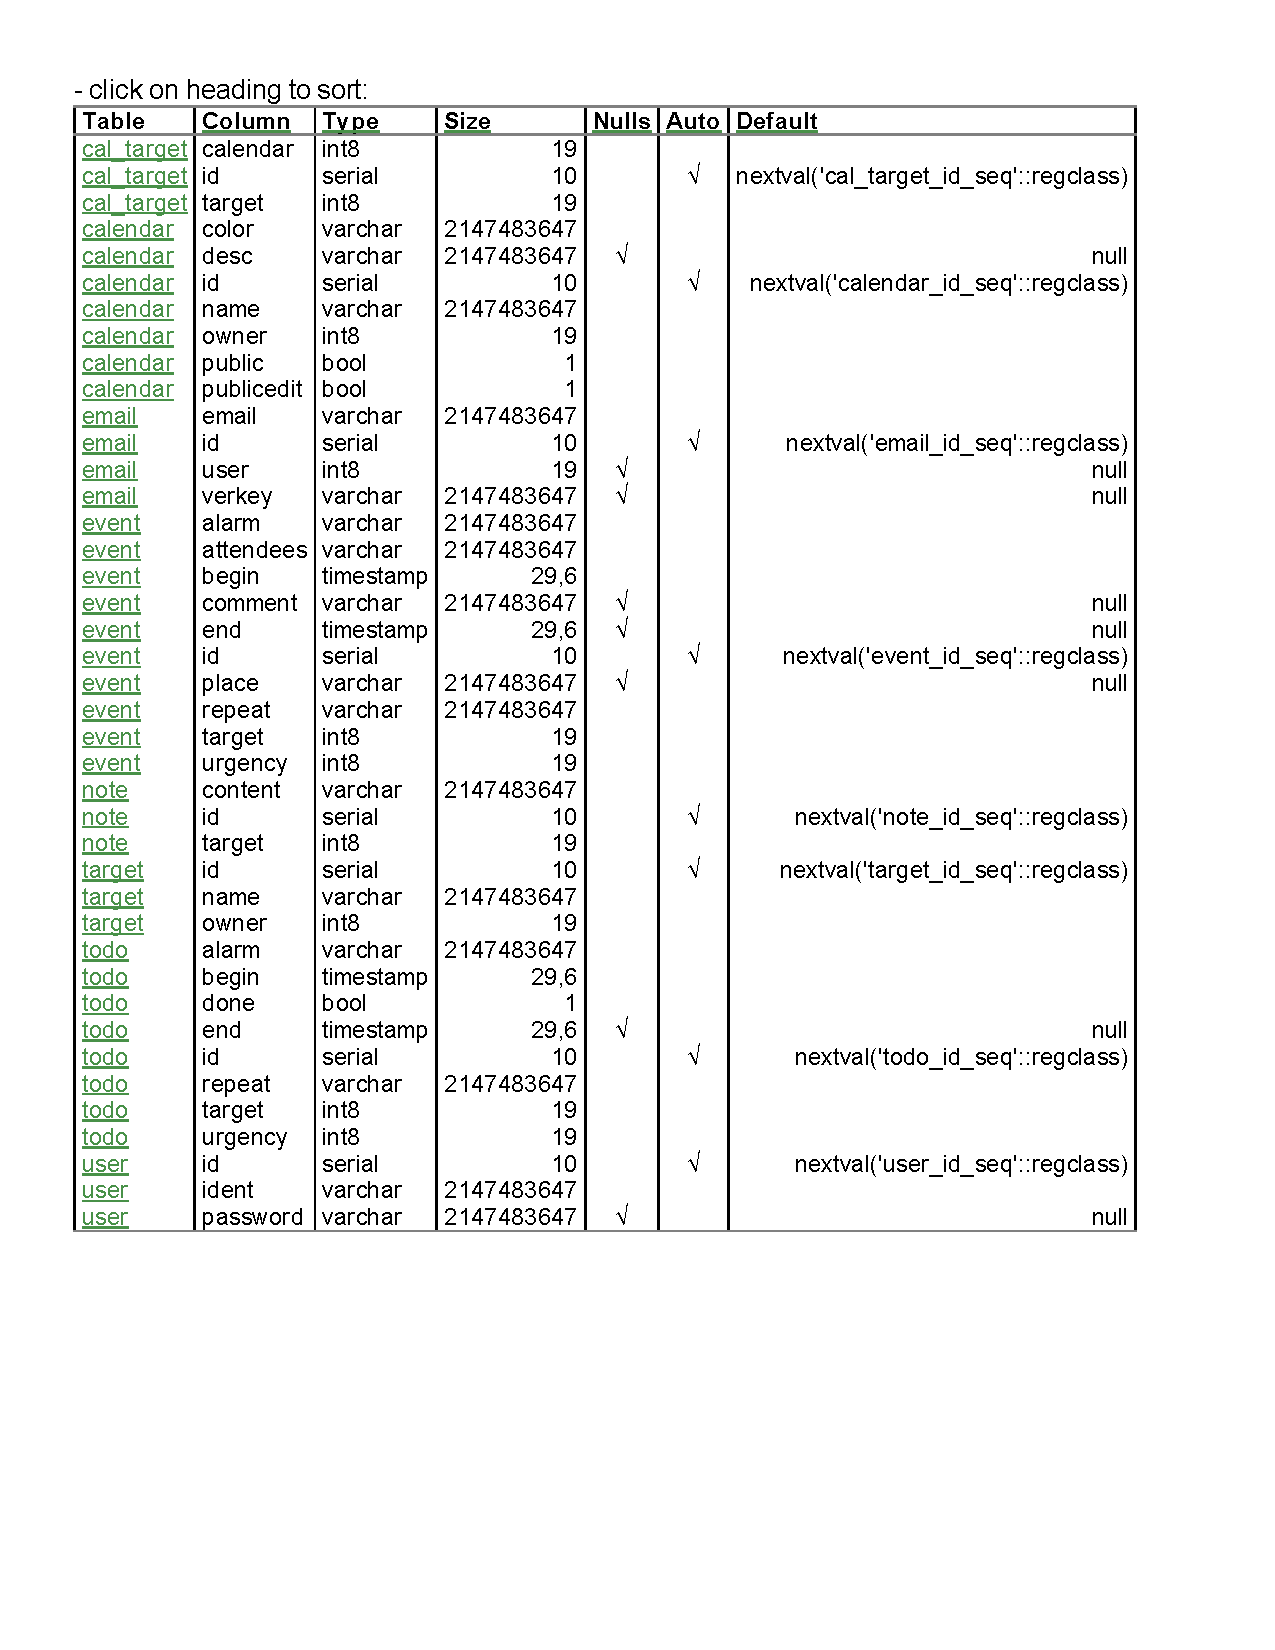
\includegraphics[clip,trim=1.2cm 7.05cm 9.21cm 1.81cm]{columns.pdf}
   \caption{Taulujen kentät ja tyypit kannassa.}
   \label{graph_columns}
\end{figure}
\clearpage

\section{Järjestelmän yleisrakenne}
Jrjestelmän pääkomponentit on sijoiteltu hakemistoihin seuraavasti.
\begin{description}
   \item[config/] \hfill\\
      Järjestelmän asetukset. \texttt{postgresql.yml} on tietokantayhteyksille
      ja \texttt{settings.yml} sisältää yleiset asetukset.  Syntaksina
      molemmissa YAML.
   \item[Handler/] \hfill\\
      Kontrollerit on sijoitettu \texttt{Handler}-kansioon.  kontrollerien
      URL:it määrätään \texttt{config/routes}-tiedostossa.
   \item[templates/] \hfill\\
      Näkymät sijaitsevat templates-kansiossa \texttt{.hamlet} ja
      \texttt{.lucius}-päätteillä.
   \item[static/] \hfill\\
      Staattinen sisältö (kääntövaiheessa).
   \item[messages/] \hfill\\
      Yesodin sisäänrakennetun i18n-tuen sanastot.
\end{description}

Lisäksi juuren \texttt{.hs}-tiedostoissa on kontrollerien käyttämä yleinen
logiikka ja tarvittavat resurssit.

\section{Järjestelmän komponentit}

\begin{description}
   \item[app/main.hs] \hfill\\
      Itse suoritettavan ohjelma lähdetiedosto (\texttt{main}-funktio).
   \item[Settings/, Application.hs, Import.hs, Model.hs, Settings.hs] \hfill\\
      Harvemmin koskemista vaativia tiedostoja, joissa toteutetaan (Yesodille)
      yleistä kontrollilogiikkaa.
   \item[CalendarTypes.hs] \hfill\\
 Kalentereihin ja kohteisiin liittyvät tyypit.
   \item[Foundation.hs] \hfill\\
      Järjestelmän keskus. Sisältää mm. autentikointinnin ja navigaatiota.
   \item[mustached-octo-happiness.cabal] \hfill\\
      Asennusohjetiedosto \textit{Cabalille}.
\end{description}

\section{Käyttöliittymä}
Käyttöliittymä on kuvattu kaaviossa~\ref{graph_ui}. Käyttöliittymässä on
yleissiirtymänavigaatio, ellei olla etusivulla, kirjautumissivulla tai
julkisella kalenterisivulla.

\begin{figure}[ht]
   \centering
   \includegraphics[width=0.7\textwidth]{ui.1}
   \caption{Käyttöliittymäkaavio. Kaikilta ei-julkisilta sivuilta pääsee
   siirtymään kalenterinäkymään, kalenteriasetuksiin sekä kirjautumaan ulos
   navigaatiopalkista.}
   \label{graph_ui}
\end{figure}

%%%%%%%%%%%%%%%%%%%%%%%%%%%%%%%%%%%%%%%%%%%%%%%%%%%%%%%%%%
\chapter{Käyttö}
\section{Asennustiedot} <++>
\section{Käynnistys- / käyttöohje} <++>

%%%%%%%%%%%%%%%%%%%%%%%%%%%%%%%%%%%%%%%%%%%%%%%%%%%%%%%%%%
\chapter{Testaus, tunnetut bugit ja puutteet \& jatkokehitysideat}
Autentikaatiossa browserId, gmail jne. failaavat, jos hashdb:llä joku on
rekisteröinyt saman spostin.

% jatko: ryhmiä, icalendar,
\bibliography{refs.bib}

\end{document}


